\chapter{Descriptions of Well-Known Classification Algorithms}
\label{chap:appendix:classification}
Here we describe the basic operation of the well-known classification algorithms used to classify our occupancy information. For those algorithms not discussed in detail in \Fref{chap:evaluation}, we also provide information on how to implement them in Weka. Based on information in Han, Kamber and Pei's ``Data Mining: Concepts and Techniques'' \cite{han2011data}.

\section{Artificial Neural Networks}
An Artificial Neural Network (ANN) uses neurons as a model for machine learning. A number of input neurons connected to the feature vectors is fed into another network of neurons (the ``hidden layer''), each of which has an activation function which determines what set of inputs will make it fire. This network then connects to a number of output neurons which can be examined to determine the network's predicted result. In the nominal result case, there is one neuron for each possible class (with each neuron being a binary yes/no), and in the numeric result case, there is one neuron without an activation function that outputs a raw numerical estimate. Neural networks can approximate functions of nearly any complexity with sufficient neurons in the correct topology, and are a commonly used classification technique.

\section{K Nearest Neighbours}
A $k$-nearest Neighbours (KNN) approach uses the topology of the training data as a means to classify future data. For each data point that requires classification, a majority vote of its $k$ nearest neighbours (defined by some distance function, typically Euclidean) in the training data determines which class it belongs to. KNN is one of the simplest machine learning algorithms, and due to its classification technique, is highly sensitive to classes that overlap. 

\section{Linear Regression}
A Linear Regression approach attempts to construct a linear equation to describe the relationship between a dependent variable (in this case, the number of people in the space), and a number of other indicator variables (in this case, the three feature vectors). Generally, the equation takes the form $y = m_1x_1 + ... + m_nx_n + c$, where each of the feature vectors ($x_n$) is multiplied by a weight ($m_n$), and then a final constant ($c$) is added to provide the final prediction.

\section{Naive Bayes}
A Naive Bayes approaches uses a simple application of Bayes' probability theorem to construct a probability of a given value belonging to a given class taking into account what is already known about the distribution of each of the classes in the data set, and the classification of those points that surround the point needing classification. One of the disadvantages of the Naive Bayes approach (and the source of its naivety) is that it assumes independence between each of the variables used for classification.

In our data, the assumption of independence of variables is not correct, as each of the features are different representations of the same underlying data. However, due to Naive Bayes' ubiquity and simplicity, it can be illuminating to see how well a very common but poorly suited classifier fares with our data set. Within Weka, we use the ``NaiveBayes'' function, which has little by way of configuration, thus is left in its default state.

\section{Support Vector Machines}
Support Vector Machines (SVM) attempt to classify data by trying to find a plane that best separates two classes in a higher dimensional space. They do this by determining ``support vectors,'' which are those data points that lie on the ``edge'' of the separation between classes, and then finding the plane that maximizes the margin between the two classes being tested. SVM is another common classification technique that we elect to investigate.

For our purposes, we use Weka's ``SMO'' function, which implements the Sequential Minimal Optimization algorithm, an efficient and recent method for training SVMs. For datasets with more than two classes (such as ours), the ``one vs. one'' method is used, whereby an SVM is created for each pair of classes, and then a method of majority voting is used to determine which class is the ultimately correct one.

\section{Decision Trees}
Decision Tree based approaches use a flow-chart of logical conditions which when met cause a data point to be classified as a specific class. Decision Tree classifiers generally use a partitioning approach whereby they split the data using a specific metric to maximize the tree's effectiveness. The advantages of Decision Trees are that they are considered to be ``white boxes,'' meaning that the result that they generate is human readable. This is useful, as in addition to the classifier providing its prediction of which class suits the data best, the tree can also be inspected to determine if the decisions it has extrapolated appear to be sensible, and even tweaked by humans if necessary.

One quite common algorithm for generating decision trees is C4.5, which is implemented by the ``J48'' function in Weka. C4.5 uses a measure of information gain, a concept rooted in information theory and entropy, to determine when to create splits in the tree. There are few configurable parameters for this approach, and for those we use the Weka defaults.

\section{0-R}
0-R is our final classification algorithm. 0-R is a simple classifier that on nominal prediction will classify all new data as belonging to the category that was most common in the training data, and on numeric prediction will classify all new data as being the mean of all test data. A 0-R classifier, clearly, is not a serious classification technique, however it is useful in establishing a baseline from which to compare all other classification results.

In Weka, the 0-R classifier is known as ``ZeroR'' and accepts no parameters.

\begin{landscape}
\chapter{Knowledge Flows}
\label{chap:knowledgeflows}

\begin{figure}[H]
\centering
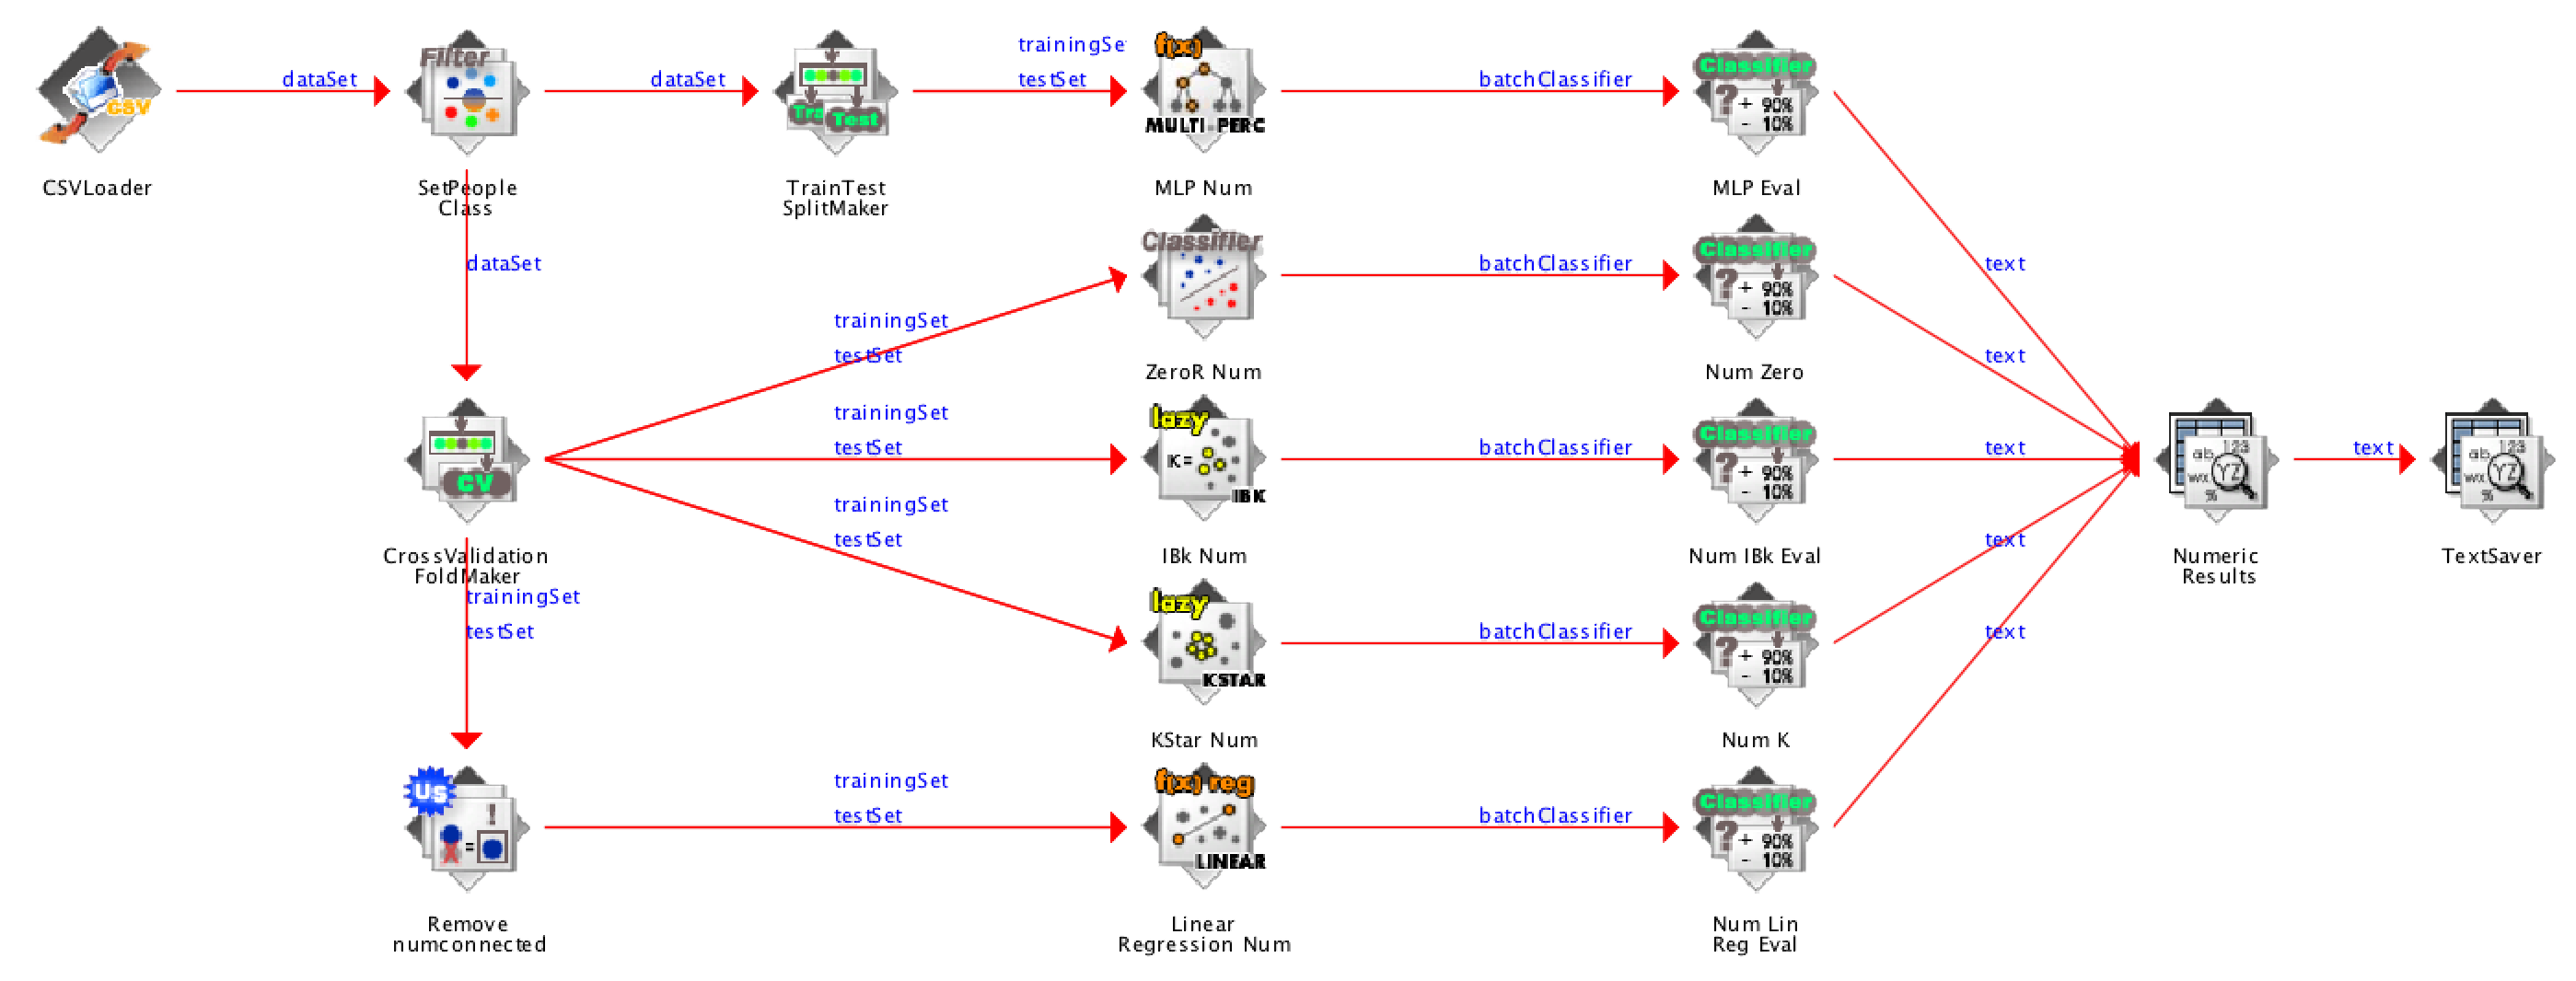
\includegraphics[width=\linewidth]{../diagrams/knowledgeflow-numeric.png}
\caption{Weka Knowledge flow for numeric classification techniques}
\end{figure}
\end{landscape}

\begin{landscape}
\begin{figure}[H]
\centering
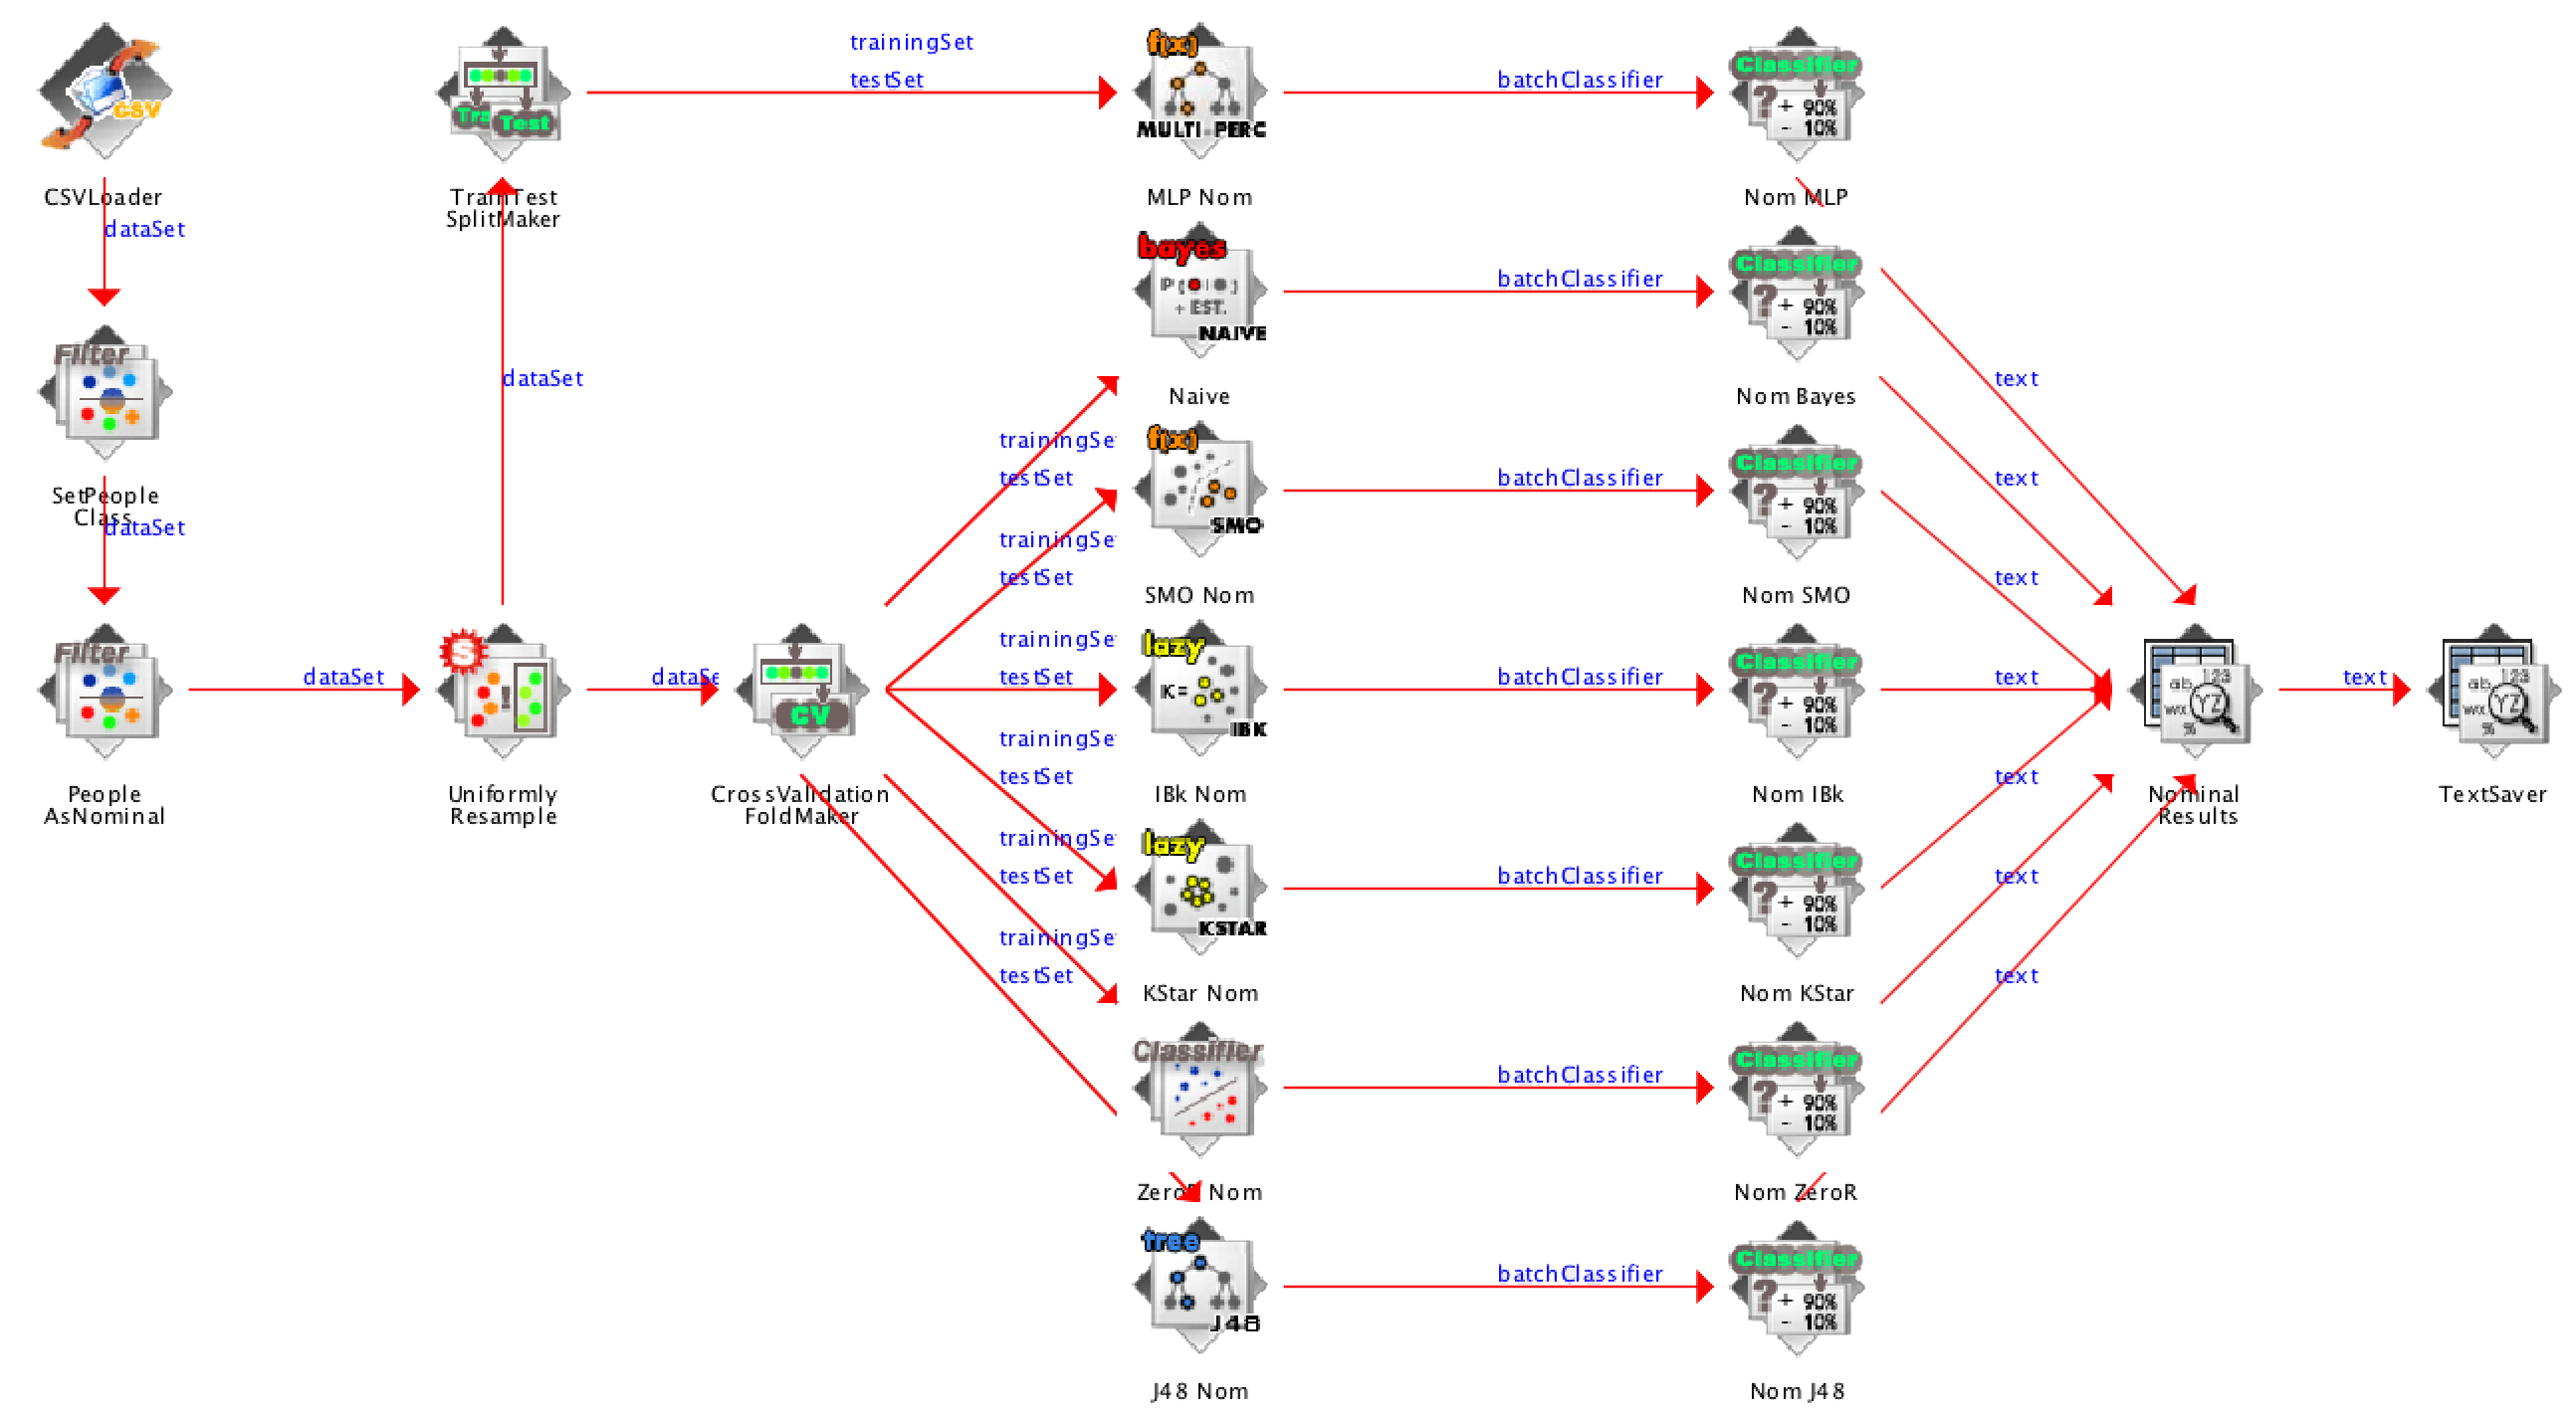
\includegraphics[width=\linewidth]{../diagrams/knowledgeflow-nominal.png}
\caption{Weka Knowledge flow for nominal classification techniques}
\end{figure}

In Weka, Knowledge Flows can be defined, which provide an easy way to replicate a series of Weka functions. We provide a unified knowledge flow at the \texttt{run\_flow.py} script to execute it on a given data set. However, we also replicate the numeric and nominal flows here (separated due to size) for those interested.
\end{landscape}

\chapter{Original Honours Proposal}
\subfile{../proposal/proposal}